\section{Phần nâng cao}
\label{sec:extensions}
Các thí nghiệm dưới đây dùng cùng mã, giao thức và bộ đánh giá như mục~\ref{sec:results}.

\subsection{CNN so với MLP}
\label{sec:cnn}
CNN gồm hai khối tích chập $3\times3$ ($16$ và $32$ kênh), mỗi khối có ReLU và gộp cực đại $2\times2$, rồi hai lớp dày đặc (mục~\ref{sec:cnn-method}). Siêu tham số được chọn bằng cùng quy trình quét trên validation.

\begin{table}[H]\centering\small
\begin{tabular}{lrr}
\toprule
 & MLP & CNN \\
\midrule
Số tham số & 535\,818 & 56\,714 \\
Kích thước ONNX (KiB) & 2094 & 223 \\
Accuracy test (\%) & 98.24 & 98.80 \\
Precision / Recall / F1 macro (\%) & 98.23 / 98.23 / 98.23 & 98.79 / 98.79 / 98.79 \\
Accuracy train $-$ test (điểm) & 1.63 & 0.60 \\
Thời gian huấn luyện (s) & 11 & 143 \\
Độ trễ một ảnh (ms) & 0.042 & 0.315 \\
Accuracy khi xoay (\%) & 96.00 & 97.46 \\
Accuracy khi dịch (\%) & 72.86 & 88.14 \\
Accuracy khi co giãn (\%) & 96.71 & 98.48 \\
Accuracy khi nhiễu Gauss (\%) & 97.31 & 98.07 \\
Accuracy khi muối tiêu (\%) & 97.56 & 97.71 \\
\bottomrule
\end{tabular}
\caption{CNN và MLP trên MNIST, cùng giao thức; mọi số lấy từ các lần chạy đã ghi. Hàng cuối: ảnh test bị biến đổi cố định (seed 999, mức mạnh hơn lúc huấn luyện), chỉ để báo cáo. Kiểm định McNemar chính xác trên dự đoán test: chỉ MLP đúng 64 ảnh, chỉ CNN đúng 120 ảnh, $p=4.4e-05$.}
\label{tab:cnn-vs-mlp}
\end{table}

\begin{figure}[tbp]
\centering
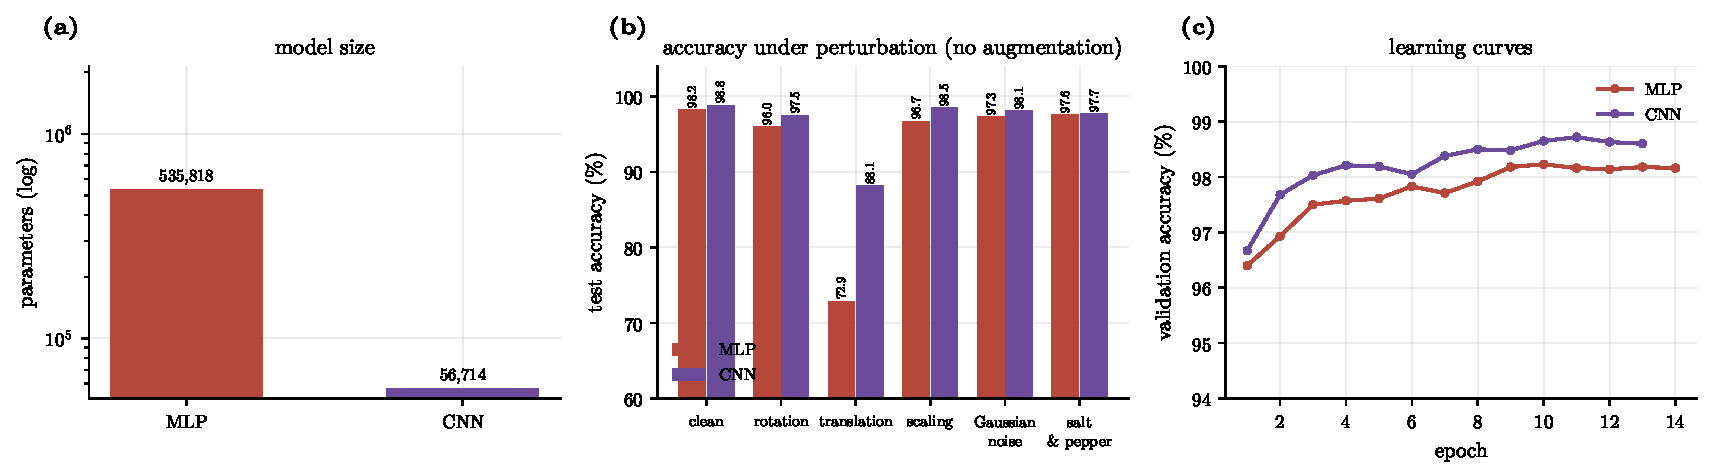
\includegraphics[width=0.92\textwidth]{../results/figures/cnn_vs_mlp.pdf}
\caption{CNN và MLP: số tham số (a), accuracy khi ảnh test bị biến đổi cố định, huấn luyện không tăng cường (b) và validation accuracy theo epoch (c).}
\label{fig:cnn-vs-mlp}
\end{figure}

CNN đạt \accTestCNN\% so với \accTestMLP\% của MLP với số tham số ít hơn $9.4$ lần, và chênh train--test nhỏ hơn ($0.60$ so với $1.63$ điểm). Khác biệt rõ nhất khi ảnh test bị dịch $3$ pixel: MLP còn $72.86\%$, CNN còn $88.14\%$ (\cref{fig:cnn-vs-mlp}b). Cái giá là thời gian: huấn luyện lâu hơn khoảng $13$ lần và mỗi ảnh chậm hơn khoảng $7$ lần (\cref{tab:cost}).

\subsection{Tăng cường dữ liệu}
\label{sec:augmentation}
Năm phép biến đổi chỉ áp dụng cho tập train, nhãn không đổi (\cref{fig:aug-examples}): xoay trong $[-15^\circ,15^\circ]$, dịch trong $[-2,2]$ pixel, co giãn trong $[0.9,1.1]$, nhiễu Gauss $\sigma=0.1$ và nhiễu muối tiêu $2\%$. Mỗi điều kiện (gốc, từng phép riêng lẻ, nhóm hình học, cả năm phép) giữ nguyên siêu tham số và chỉ thêm một bản sao biến đổi của mỗi ảnh train ($100\,000$ ảnh); chạy 3 seed (MLP) hoặc 2 seed (CNN). Điều kiện được chọn theo validation; để đo độ bền, tập test được biến đổi mạnh hơn lúc huấn luyện. Vì điều kiện tăng cường có dữ liệu gấp đôi điều kiện gốc, ảnh hưởng của loại biến đổi và của lượng dữ liệu bị lẫn.

\begin{figure}[tbp]
\centering
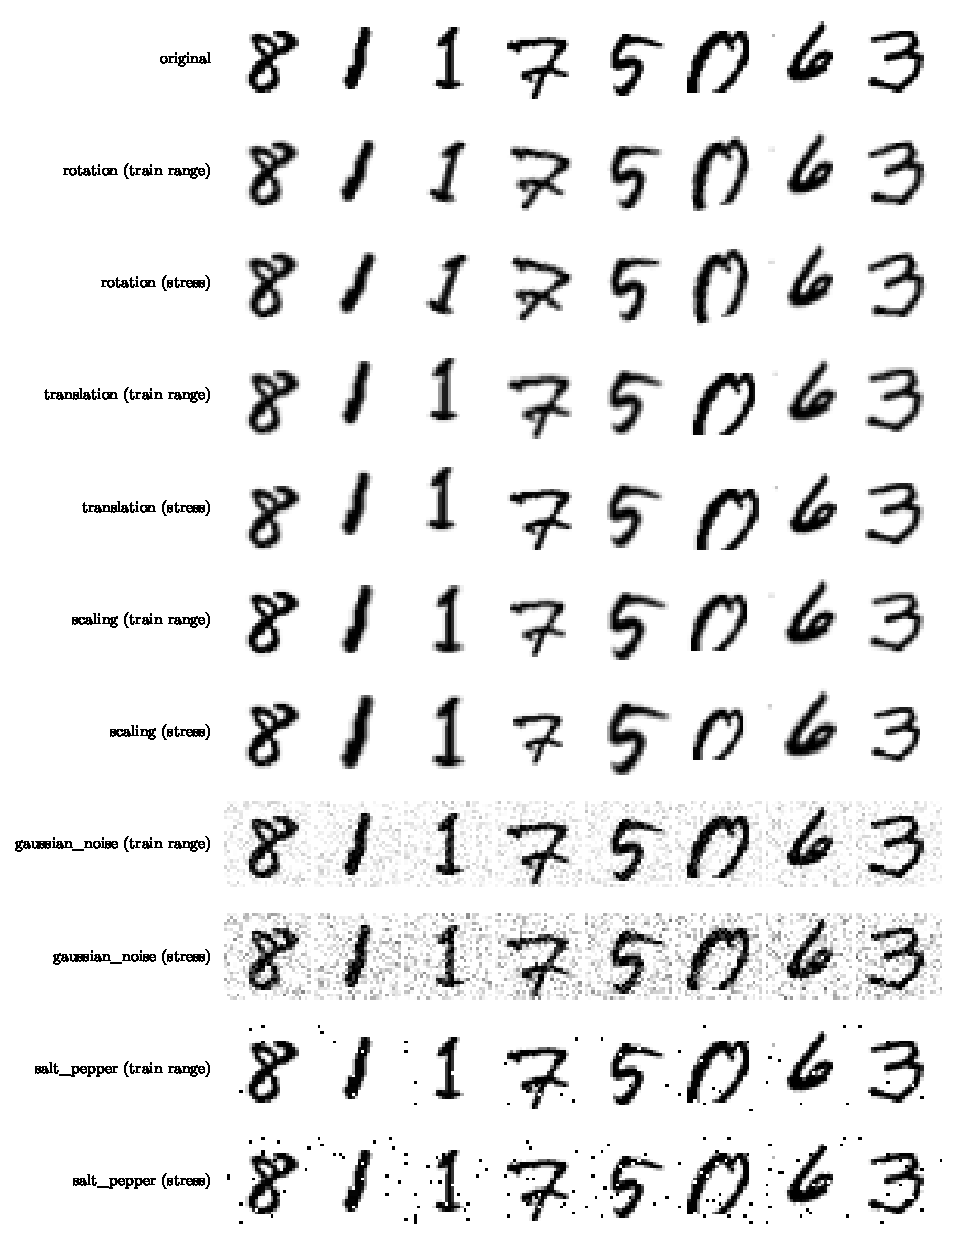
\includegraphics[width=0.85\textwidth]{../results/figures/augmentation_examples.pdf}
\caption{Ảnh gốc và từng phép biến đổi ở mức huấn luyện và mức kiểm tra độ bền.}
\label{fig:aug-examples}
\end{figure}

\begin{table}[H]\centering\small
\begin{tabular}{lrrrr}
\toprule
 & \multicolumn{2}{c}{MLP (3 seed)} & \multicolumn{2}{c}{CNN (2 seed)} \\
\cmidrule(lr){2-3}\cmidrule(lr){4-5}
Điều kiện & $\Delta$ val (điểm) & Test (\%) & $\Delta$ val (điểm) & Test (\%) \\
\midrule
Không tăng cường & -- & 98.02 & -- & 98.82 \\
Xoay & +0.57 $\pm$ 0.47 & 98.48 & +0.23 $\pm$ 0.01 & 99.17 \\
Dịch chuyển & +0.54 $\pm$ 0.55 & 98.41 & +0.22 $\pm$ 0.03 & 99.17 \\
Co giãn & +0.42 $\pm$ 0.45 & 98.33 & +0.20 $\pm$ 0.01 & 99.06 \\
Nhiễu Gauss & +0.38 $\pm$ 0.42 & 98.35 & +0.19 $\pm$ 0.20 & 99.06 \\
Nhiễu muối tiêu & +0.37 $\pm$ 0.40 & 98.32 & +0.17 $\pm$ 0.06 & 99.00 \\
Hình học (xoay, dịch, co giãn) & +0.31 $\pm$ 0.33 & 98.24 & +0.25 $\pm$ 0.16 & 99.20 \\
Cả năm phép & +0.09 $\pm$ 0.40 & 98.11 & +0.31 $\pm$ 0.01 & 99.25 \\
\bottomrule
\end{tabular}
\caption{Tăng cường dữ liệu với cấu hình đã chọn: $\Delta$ là hiệu validation accuracy so với điều kiện gốc \emph{cùng seed} (trung bình $\pm$ độ lệch chuẩn mẫu của hiệu), ``Test'' là accuracy test sạch trung bình trên các seed. Mỗi điều kiện tăng cường dùng $100\,000$ ảnh train, điều kiện gốc $50\,000$.}
\label{tab:augmentation}
\end{table}


\Cref{tab:augmentation} cho thấy với MLP, mọi điều kiện tăng validation $0.09$--$0.57$ điểm nhưng cùng bậc với độ lệch chuẩn ghép cặp ($0.33$--$0.55$), nên chưa khẳng định được tác dụng trên ảnh sạch; với CNN, test sạch tăng từ $98.82\%$ lên $99.00$--$99.25\%$ (chỉ 2 seed). Tác dụng rõ nhất là độ bền với đúng loại biến đổi: huấn luyện với phép dịch nâng accuracy của MLP trên ảnh bị dịch từ $72.1\%$ lên $94.5\%$. Một phép tăng cường cũng có thể làm giảm độ bền ở loại khác: với CNN, chỉ dùng phép dịch hoặc nhóm hình học làm accuracy trên ảnh nhiễu Gauss mạnh giảm từ $97.2\%$ xuống $95.0\%$ và $93.6\%$.

\subsection{Fashion-MNIST và EMNIST Digits}
\label{sec:datasets}
Fashion-MNIST \citep{xiao2017} gồm ảnh $28\times28$ của $10$ loại quần áo; EMNIST Digits \citep{cohen2017} gồm chữ số viết tay ($240\,000$ ảnh train, $40\,000$ ảnh test; nhóm lấy $60\,000$ ảnh train chia $50\,000/10\,000$ và giữ nguyên $40\,000$ ảnh test). Mỗi bộ dữ liệu có phép chia, hằng số chuẩn hóa và siêu tham số riêng (quét rút gọn, một seed).

\begin{table}[tbp]\centering\small
\begin{tabular}{lrrr}
\toprule
Mô hình & MNIST & Fashion-MNIST & EMNIST Digits \\
\midrule
Gaussian NB & 81.32 / 81.16 & 67.27 / 66.03 & 80.03 / 80.13 \\
Softmax regression & 92.52 / 92.42 & 84.27 / 84.18 & 93.81 / 93.81 \\
MLP & 98.24 / 98.23 & 88.59 / 88.55 & 98.36 / 98.36 \\
AdaBoost-SAMME & 97.60 / 97.58 & 84.74 / 84.88 & 97.38 / 97.38 \\
CNN & 98.80 / 98.79 & 88.49 / 88.48 & 98.64 / 98.64 \\
\bottomrule
\end{tabular}
\caption{Accuracy / macro-F1 trên tập test (\%) của từng bộ dữ liệu; mỗi bộ dữ liệu có phép chia train/validation/test riêng, siêu tham số chọn riêng trên validation của bộ đó (quét rút gọn cho Fashion-MNIST và EMNIST Digits). Không so sánh chéo giữa các bộ dữ liệu.}
\label{tab:datasets}
\end{table}


Thứ hạng ổn định ở hai bộ chữ số (Naïve Bayes $<$ softmax $<$ AdaBoost $<$ MLP $\le$ CNN, \cref{tab:datasets}) nhưng đổi ở Fashion-MNIST: MLP và CNN ngang nhau ($88.59$ và $88.49\%$) và Naïve Bayes giảm còn $67.27\%$. Mô hình huấn luyện trên MNIST rồi đánh giá trên EMNIST Digits (cùng 10 chữ số) đều giảm (\cref{tab:cross-eval}): CNN giảm ít nhất ($6.5$ điểm), softmax nhiều nhất ($40.2$ điểm). Fashion-MNIST dùng nhãn khác nên không có phép kiểm tra chéo hợp lệ với bộ chữ số. Nhóm chưa thử bộ chữ số viết tay tiếng Việt.

\begin{table}[H]\centering\small
\begin{tabular}{lrr}
\toprule
Mô hình & Huấn luyện trên MNIST & Huấn luyện trên EMNIST Digits \\
\midrule
Gaussian NB & 49.80 & 80.03 \\
Softmax regression & 53.59 & 93.81 \\
MLP & 76.70 & 98.36 \\
CNN & 92.15 & 98.64 \\
AdaBoost-SAMME & 73.69 & 97.38 \\
\bottomrule
\end{tabular}
\caption{Accuracy (\%) trên $40\,000$ ảnh test của EMNIST Digits. Cột giữa là mô hình huấn luyện trên MNIST (dùng hằng số chuẩn hóa của MNIST) đánh giá trực tiếp; cột phải là mô hình huấn luyện trên EMNIST Digits. Đây là hai mô hình khác nhau.}
\label{tab:cross-eval}
\end{table}


\subsection{Giao diện demo}
\label{sec:demo}
Trang web (React, TypeScript, ONNX Runtime Web \citep{onnxruntime}) cho phép vẽ hoặc chọn ảnh, chọn bộ dữ liệu và một trong năm mô hình rồi xem dự đoán chạy ngay trong trình duyệt. Mô hình được xuất sang ONNX (riêng AdaBoost dùng tệp nhị phân của các cây) và đối chiếu với mô hình Python: Gaussian NB: sai lệch xác suất lớn nhất $1.4e-04$\, trùng nhãn 100.00\% trên 2\,000 ảnh; Softmax regression: sai lệch xác suất lớn nhất $3.4e-06$\, trùng nhãn 100.00\% trên 2\,000 ảnh; MLP: sai lệch xác suất lớn nhất $1.7e-06$\, trùng nhãn 100.00\% trên 2\,000 ảnh; AdaBoost-SAMME: sai lệch xác suất lớn nhất $0.0e+00$\, trùng nhãn 100.00\% trên 2\,000 ảnh; CNN: sai lệch xác suất lớn nhất $7.2e-07$\, trùng nhãn 100.00\% trên 2\,000 ảnh%
. Mô hình nằm trên Hugging Face Hub, được ghim theo mã commit. Chức năng ``nhìn vào bên trong'' vẽ lại phép tính của chính mô hình đã triển khai; đó là trực quan hóa phép tính, không phải lời giải thích vì sao mô hình quyết định như vậy.
